\documentclass[12pt,a4paper,titlepage,openany, oneside]{report}
\usepackage[utf8]{inputenc}
\usepackage[T1]{fontenc}
\usepackage[french]{babel}
\usepackage[top=1.5cm, bottom=4cm]{geometry}
\usepackage{fancyhdr, graphicx, array, hyperref}
\usepackage{glossaries}

%\usepackage[onehalfspacing]{setspace}
%\usepackage{pdfpages}

\pagestyle{fancy}

\title{\textsc{\textbf{Conception\\Interpréteur du langage LIR}}}
\date{}
\author{Nicolas \textsc{Caminade} \and Sylvan \textsc{Courtiol} \and
    Pierre \textsc{Debas} \and Heïa \textsc{Dexter} \and Lucàs
    \textsc{Vabre} }
\begin{document}
    \lhead{\leftmark}
    \rhead{
        
\includegraphics[width=2cm]{img/logoiut}
    }

    \cfoot{\thepage}
    \headheight = 2cm
    \headsep = 0.5cm

    \begin{titlepage}
        \fontfamily{pag}\selectfont

        \begin{center}\normalsize
            \MakeUppercase{IUT de Rodez \hfill Département informatique
                \hfill INFO1 2020-2021}
        \end{center}
        \vspace*{0.1cm}
        \hrule
        \vspace*{0.2cm}
        \begin{flushright}
            
\includegraphics[width=4cm]{img/logoiut}
        \end{flushright}
        \vspace*{2cm}
        \begin{flushright}\Huge
            \textsc{\textbf{Conception\\Interpréteur du langage LIR}}
        \end{flushright}
        \hrule
        \begin{flushleft}
            \MakeUppercase{Projet proposé par Frédérique Barrios}
        \end{flushleft}
        \vspace*{2cm}
        \begin{center}\Large
            Nicolas \textsc{Caminade}, Sylvan \textsc{Courtiol},\\
            Pierre \textsc{Debas}, Heïa \textsc{Dexter}, \\
            Lucàs \textsc{Vabre}
        \end{center}
        \vfill
        \begin{center}\normalsize
            \MakeUppercase{Projet tuteuré --- Semestre 2}
        \end{center}
    \end{titlepage}

    \renewcommand\rmdefault{pag}
    \fontfamily{pag}\selectfont
    \renewcommand{\sfdefault}{pag}

    % Sommaire
    \renewcommand{\contentsname}{Sommaire}
    \tableofcontents

    \setcounter{part}{2} % La conception est la troisième partie du dossier

    \part{Conception}

    \chapter{Itération 1}

    \par L'objectif de l'itération 1 était un prototype qui devait premièrement pouvoir se lancer et s'éteindre. De plus le prototype devait pouvoir gérer (mémorisation, affectation) des données de type chaines. Les commandes debut, defs, fin et l'instruction var ont donc été ajoutés afin d'obtenir ces fonctionnalités.

\section{Paquetage interpreteurlir.donnees.litteraux}
\begin{center}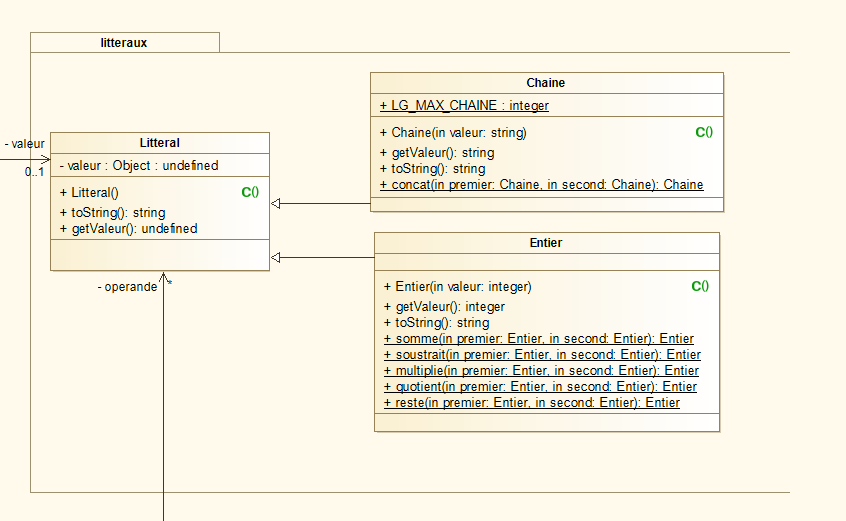
\includegraphics[scale=0.75]{./img/COO/COO_prototype_1/PackageLitteraux}\end{center}
\par Le choix de conception des littéraux a été une classe parente Litteral qui permet d'englober tous les types de données du programme.
La classe Entier a été détaillé dans la conception cependant elle n'a pas été codée à cette itération pour se concentrer sur les chaînes.
Les littéraux sont immuables pour permettre leur passage sans problème.

\section{Paquetage interpreteurlir.donnees}
\begin{center}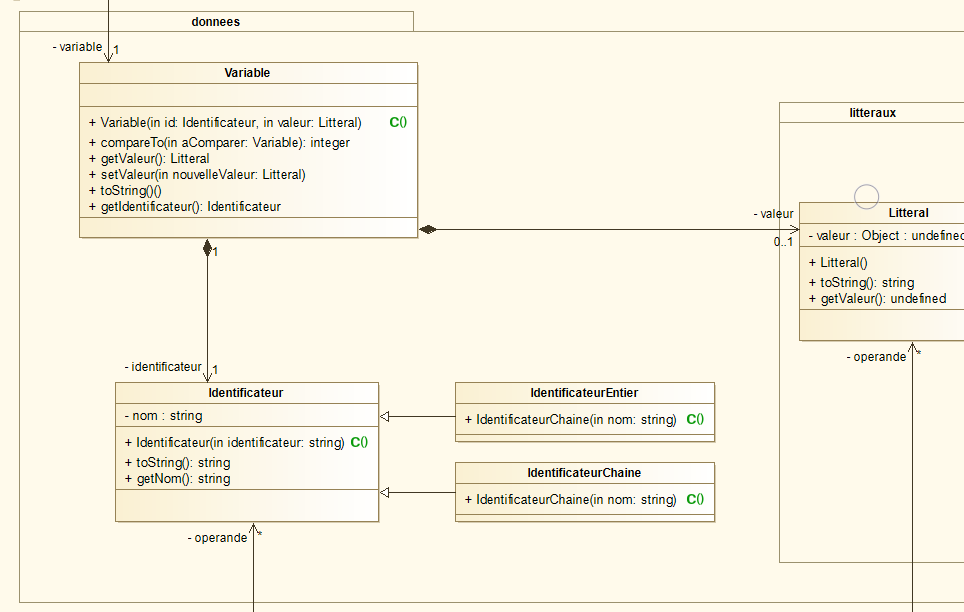
\includegraphics[scale=0.65]{./img/COO/COO_prototype_1/PackageDonnees}\end{center}
\par Pour les données une classe variable a été choisie composée d'un littéral et d'un identificateur.
L'identificateur a comme classes dérivées les deux types affectables du projet soit les entiers et les chaînes.

\section{Paquetage interpreteurlir.expressions}
\begin{center}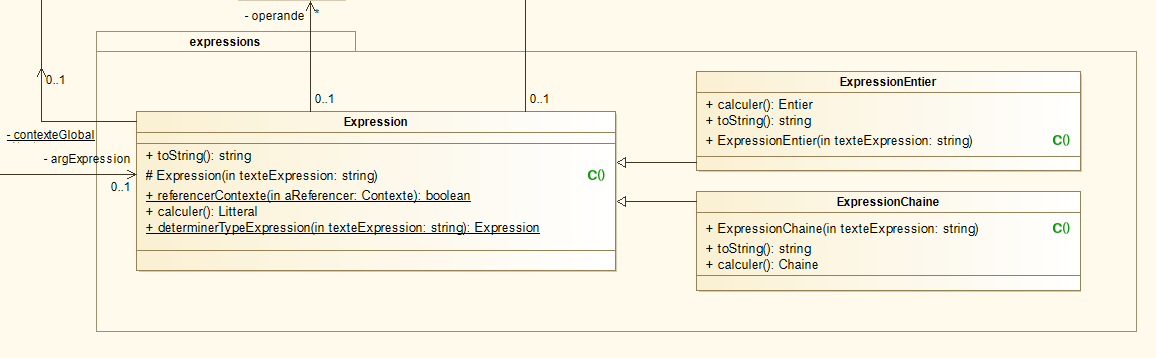
\includegraphics[scale=0.60]{./img/COO/COO_prototype_1/PackageExpressions}\end{center}
\par Comme pour le reste de notre conception les expressions sont typées et sont une spécialisation d'une classe Expression générale regroupant les comportements communs. Une méthode de classe d'Expression permet de créer le bon type d'expression.

\section{Paquetage interpreteurlir.motscles}
\begin{center}\includegraphics[scale=0.60]{./img/COO/COO_prototype_1/PackageMotscles}\end{center}
\par La conception de l'itération 1 contient ce qui devait être faits lors de cette itération à quelques détaille près comme la classe InstructionAffiche qui n'a pas été codée car non nécessaire aux fonctionnalités choisies.
L'itération 1 voulait permettre de manier des chaînes il fallait donc que les commandes connaissent le contexte contenant les variables. La solution choisie a été une attribut d'instance dans Commande initialiser à la construction de la commande par passage de la référence du contexte global par le constructeur. Une instance de commande correspond à un objet ayant toutes les informations nécessaire pour être exécuté (String arguments dans le constructeur). Les commandes et instructions fonctionnent en 2 temps, la construction qui valide les arguments et créer les éléments nécessaires à l'exécution puis l'exécution qui est la réalisation du comportement de la commande.

\section{Paquetage interpreteurlir}
\begin{center}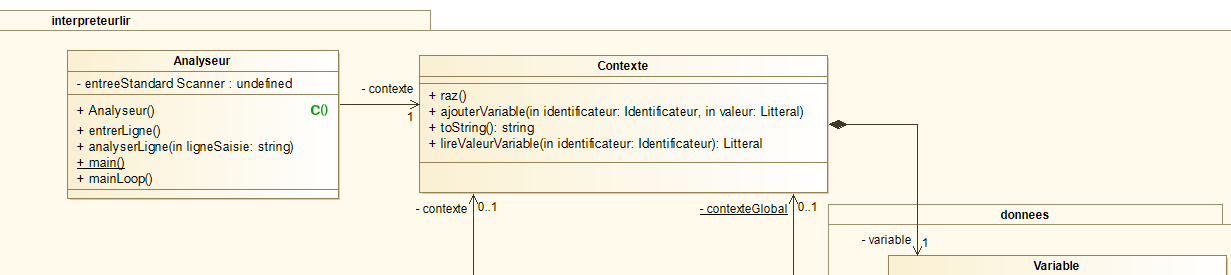
\includegraphics[scale=0.60]{./img/COO/COO_prototype_1/PackageInterpreteurlir}\end{center}
\par Le contexte regroupe l'entièreté des variables définies dans la session courante. Une variable n'est accessible que par l'intermédiaire du contexte grâce à l'identificateur qui sert de clé. L'Analyseur est la classe qui permet le fonctionnement de tout. Une mainLoop permet de demander en continue une ligne à l'utilisateur puis celle-ci est analyser, à partir du mot clé une commande/instruction est crée en passant le reste de la ligne en argument. L'analyse des arguments se fait au niveau le plus interne possible (Analyseur analyse le mot cle, la commande les arguments qui construit ensuite les éléments dont elle a besoin qui s'occupe eux-mêmes de vérifier leur validité à la construction). Si une erreur dans la ligne à interprété est détecté alors une InterpreteurException est levée et se propage jusqu'à l'analyseur qui affiche l'erreur.

\section{Illustration avec des diagrammes d'objets}
\begin{center}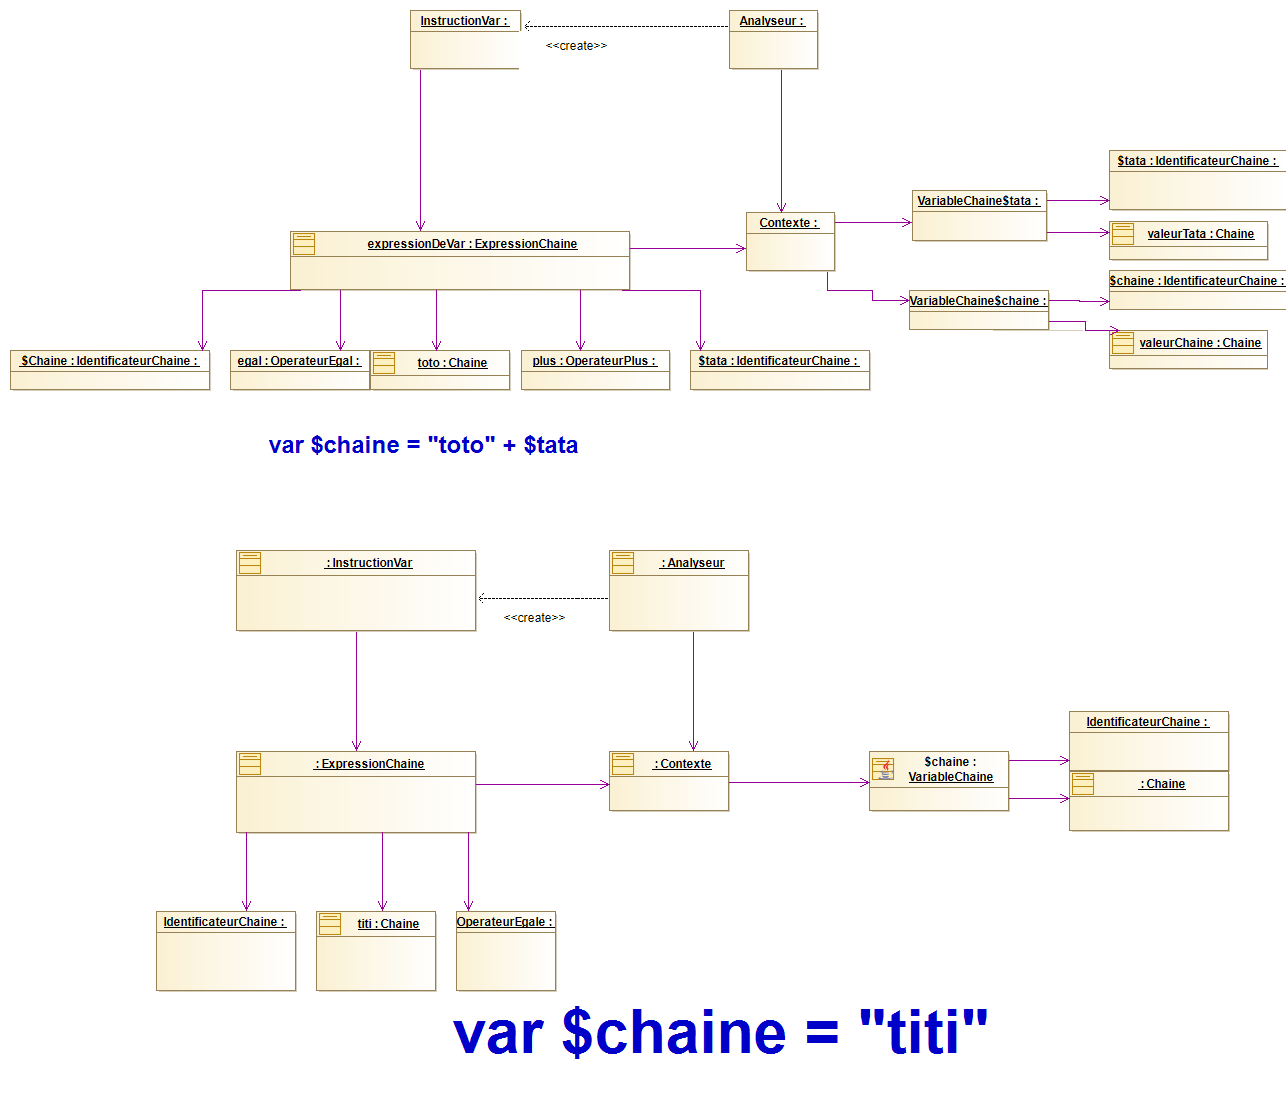
\includegraphics[scale=0.50]{./img/COO/COO_prototype_1/Objet}\end{center}
\par Voici des diagrammes qui ont été faits pendant la réflexion de cette conception. Ils permettent d'illustrer le fait qu'une instruction créer les éléments dont elle a besoin. Seul changement dans la conception par rapport à ces diagrammes : les opérateurs sont gérer en interne des instructions (il n'y pas de classe Operateur).

    \normalsize
    \chapter{Itération 2}

    \par L'itération 2 avait pour objectif d'ajouter le type entier. Puis il fallait pourvoir faire une programme, c'est-à-dire des instructions ordonnées avec des étiquettes exécutables plus tard. Pour compléter les objectifs de cette itération certaines commandes et instructions ont été réalisées (efface, liste, lance/affiche, entre, vaen, procedure, stop, retour).

\section{Diagrammes d'objets}
Comme conseillé par notre tuteur, nous avons commencé la conception de l'itération 2 par des diagrammes d'objets. Ci-dessous quelques exemples.
\par
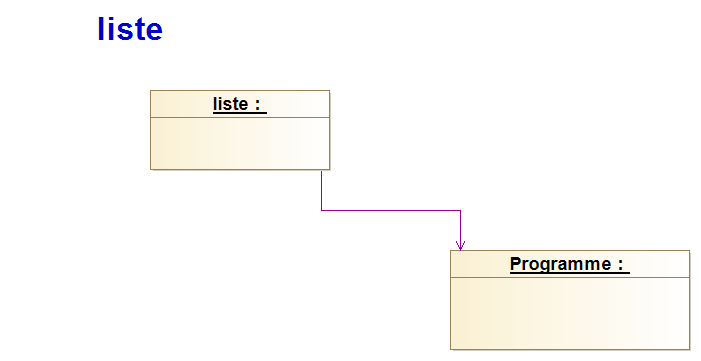
\includegraphics[scale=0.5]{./img/COO/COO_prototype_2/digrammesObjet/Diagramme d'objet la commande liste}
\par Le premier montre que la commande liste fait appel au programme (contenant les lignes de codes constituant un programmes) pour exécuter son comportement.
\par
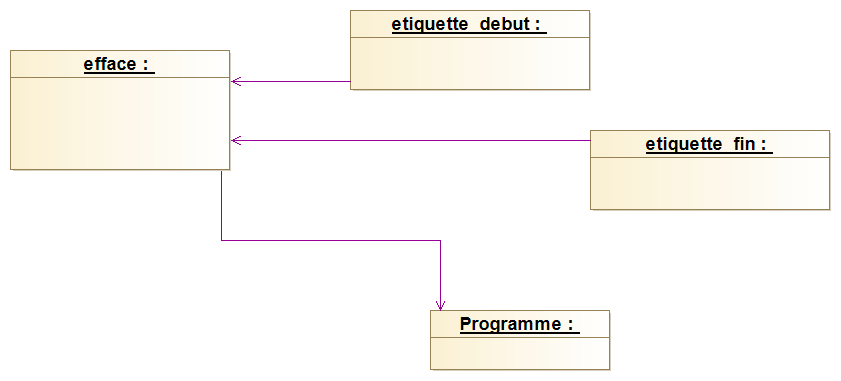
\includegraphics[scale=0.5]{./img/COO/COO_prototype_2/digrammesObjet/Diagramme d'objet de la commande efface}
\par La commande efface connait donc les deux étiquettes qui définissent sont comportement spécifique d'instance. Pour sont exécution elle doit connaitre le programme global de la session courante de l'interpréteur LIR.

\section{Paquetage interpreteurlir.donnees(.litteraux)}
\par Les paquetages donnees et litteraux n'ont que très peu changé en conception mais les classe liées aux entiers ont été codés pendant cette itération.

\section{Paquetage interpreteurlir.expressions}
\par Comme pour les données, pas de changement de conception mais programmtion de ExpressionEntier.

\section{Paquetage interpreteurlir.programmes}
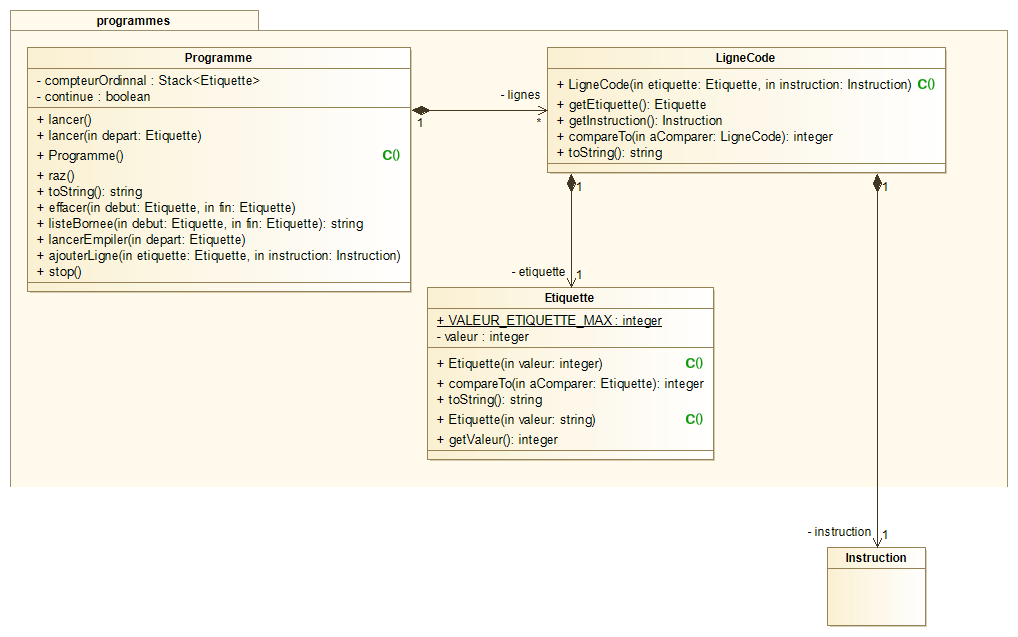
\includegraphics[scale=0.5]{./img/COO/COO_prototype_2/PackageProgrammes}
\par Premièrement la classe étiquette permet d'ordonner les lignes de codes. Le Programme contient des méthodes pour tous les comportement qu'il doit réaliser ce qui permet de les intégrés en interne ce qui rend leur usage plus simple pour les commandes et instructions. Seul la méthode vaen est absente de la conception car nous nous sommes rendu compte qu'elle était nécessaire pendant la programmation. Autre changement, le programme doit enregistrés les lignes de codes. La conception montre une classe LigneCode prévue à cet effet cependant sur le conseil de notre tuteur nous avons utilisé une TreeMap<Etiquette, Instruction> ce qui a rendu LigneCode obsolète. La classe avait été programmée et testée mais nous l'avons supprimée car TreeMap était une meilleur solution.

\section{Paquetage interpreteurlir.motscles} 
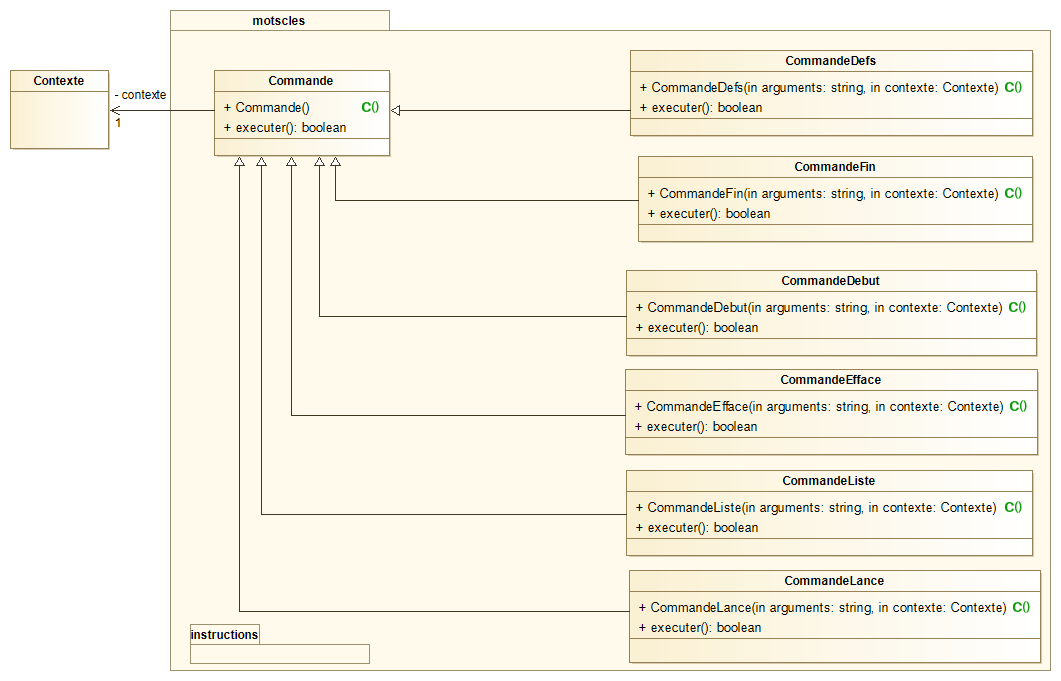
\includegraphics[scale=0.45]{./img/COO/COO_prototype_2/PackageCommande}
\par Les commandes à ajouter à cette itération ont été ajoutée à la conception en suivant le même principe de la dualité construction/exécution. Seul changement notable (non montré dans le diagramme car décidé pendant la programmation), l'ajout du programme nécessite que les commandes connaissent celui-ci. Après une longue réflexion nous avons choisis de le déclaré comme attribut protected dans la classe Commande et de le référencer au lancement de l'interpréteur sans savoir si c'était un bon choix ou non.

\section{Paquetage interpreteurlir.motscles.instructions} 
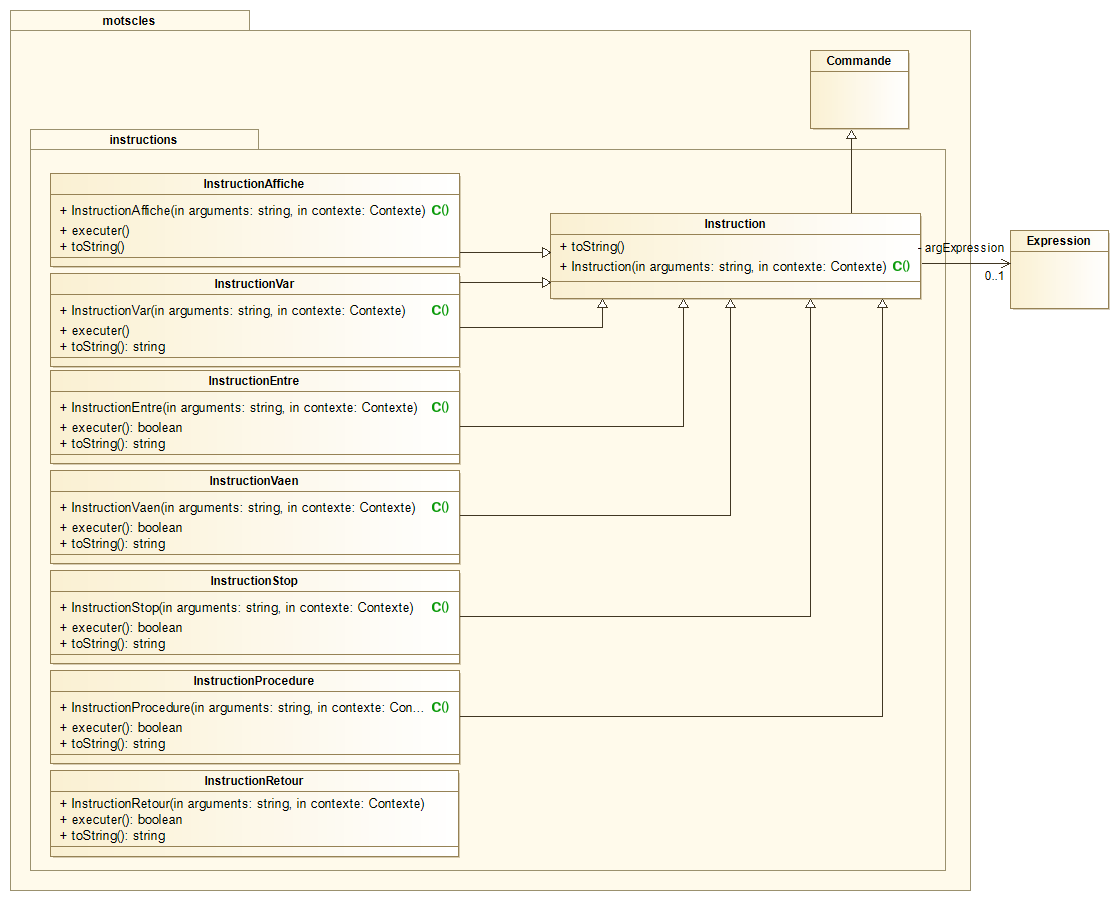
\includegraphics[scale=0.45]{./img/COO/COO_prototype_2/PackageInstruction}
\par Aucun changement notable, seulement ajout des nouvelles instructions.

\section{Paquetage interpreteurlir}
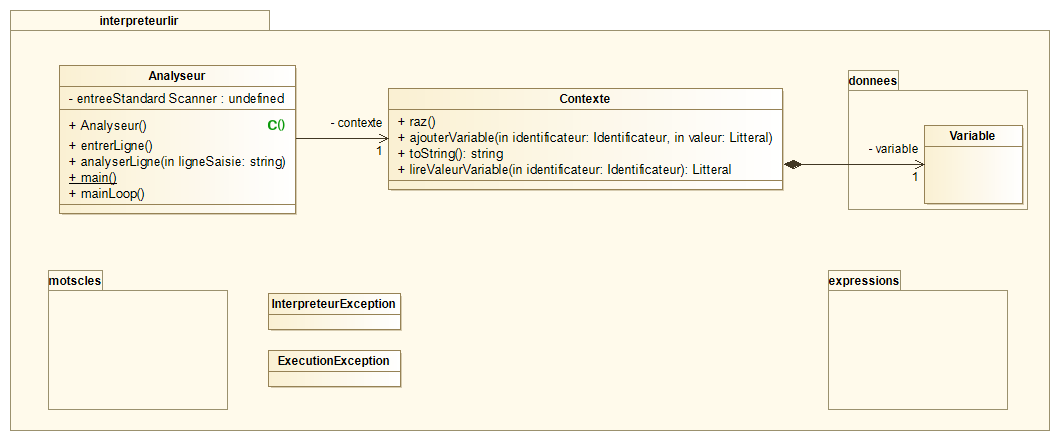
\includegraphics[scale=0.45]{./img/COO/COO_prototype_2/PackageInterpreteurlir}
\par Ajout de l'exception ExecutionException lancée pour une erreur à l'exécution comme une division par 0 (contrairement à l'InterpreteurException qui est lancée à la construction). Elle également affichée par l'Analyseur.

    \chapter{Itération 3}


    \par L'itération 3 à ajoutée les expressions booléennes avec l'instruction si vaen. Et les commandes permettent d'enregistrer et charger un programme LIR dans l'interpréteur (commande charge et sauve).

\section{Diagrammes d'objets}
\begin{center}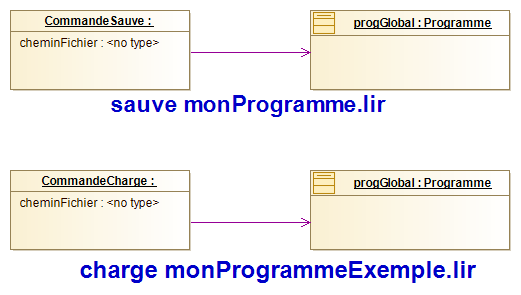
\includegraphics[scale=0.80]{fichiers/dossierPartieConception/img/COO/COO_prototype_3/digrammesObjet/charge}\end{center}
\par Les commandes sauve et charge sont liées au programme pour pouvoir charger ou récupérer des lignes de codes. Ces commandes connaissent une chaînes de texte correspondant au chemin du fichier.
\par
\begin{center}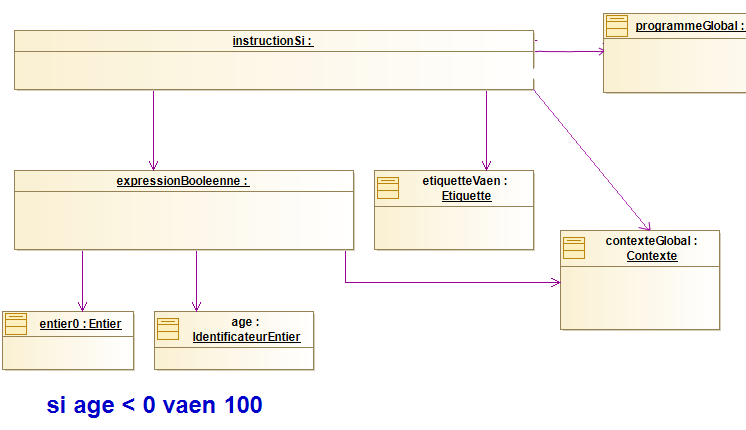
\includegraphics[scale=0.75]{fichiers/dossierPartieConception/img/COO/COO_prototype_3/digrammesObjet/siVaen}\end{center}
\par L'instruction si a besoin pour fonctionner d'une ExpressionBooleenne et de connaitre le contexte pour chercher les valeurs des variables à comparer. Elle doit connaitre l'étiquette où aller si la condition est vraie et donc du programme pour appeler la méthode du programme vaen.

\section{Paquetage interpreteurlir.donnees(.litteraux)}
\begin{center}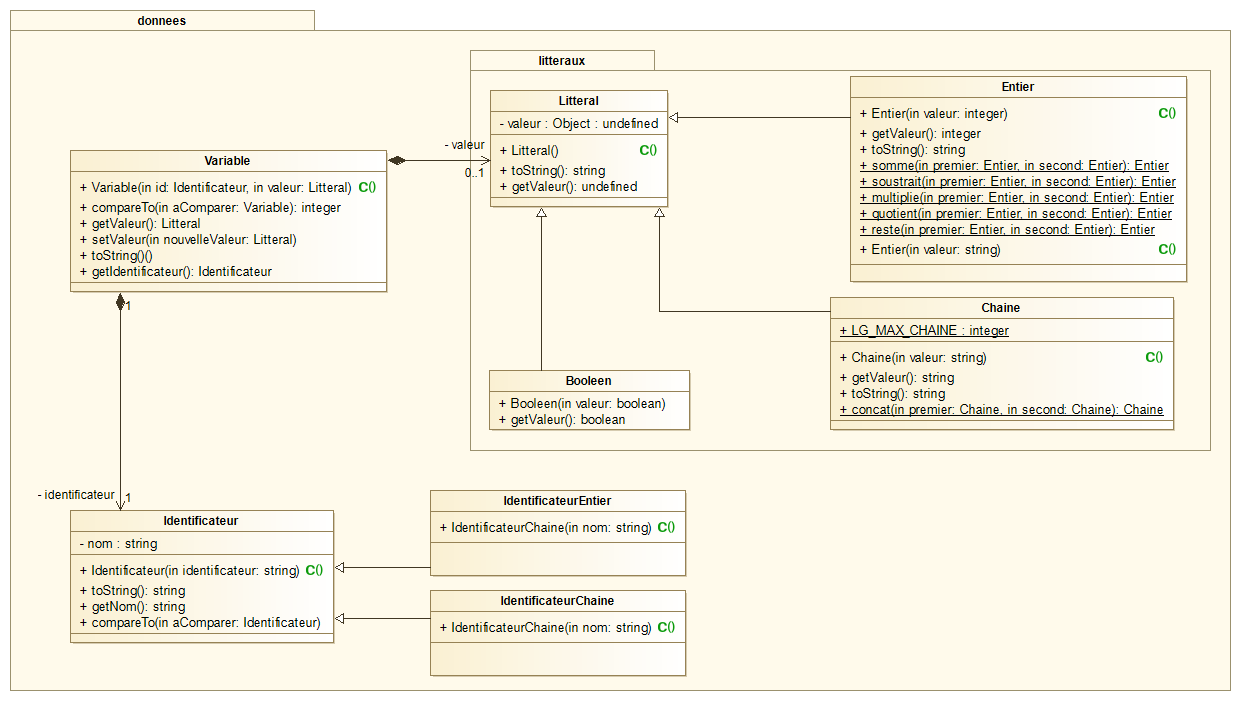
\includegraphics[scale=0.40]{fichiers/dossierPartieConception/img/COO/COO_prototype_3/PackageDonnees}\end{center}
\par Le type booléen hérite de Litteral pour garder la logique de Litteral pouvant référencer chaque type de valeur du programme.

\section{Paquetage interpreteurlir.expressions}
\begin{center}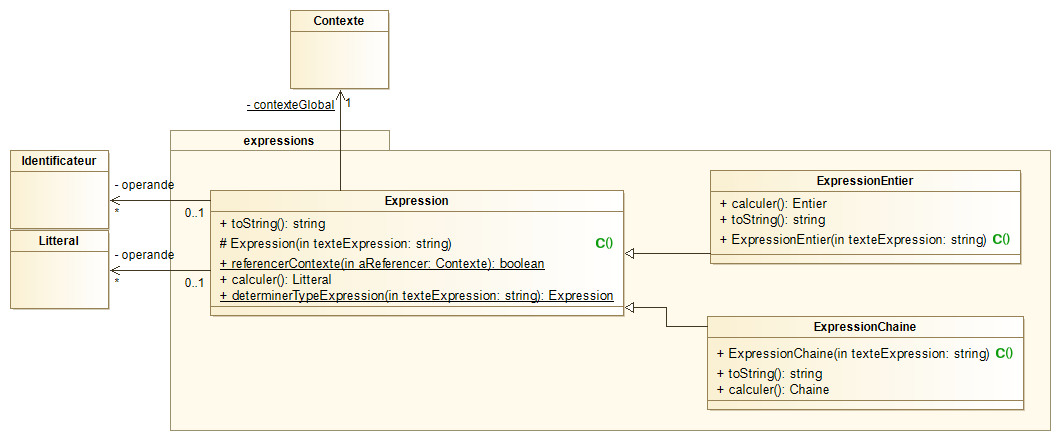
\includegraphics[scale=0.45]{fichiers/dossierPartieConception/img/COO/COO_prototype_3/PackageExpression}\end{center}
\par L'expression booléenne ne s'obtient pas avec la méthode determinerExpression car celle-ci est utilisée que par si vaen qui utilise que ce type d'expression. Le constructeur d'ExpressionBooleenne est donc utilisé directement.

\section{Diagramme de classes général}
\begin{center}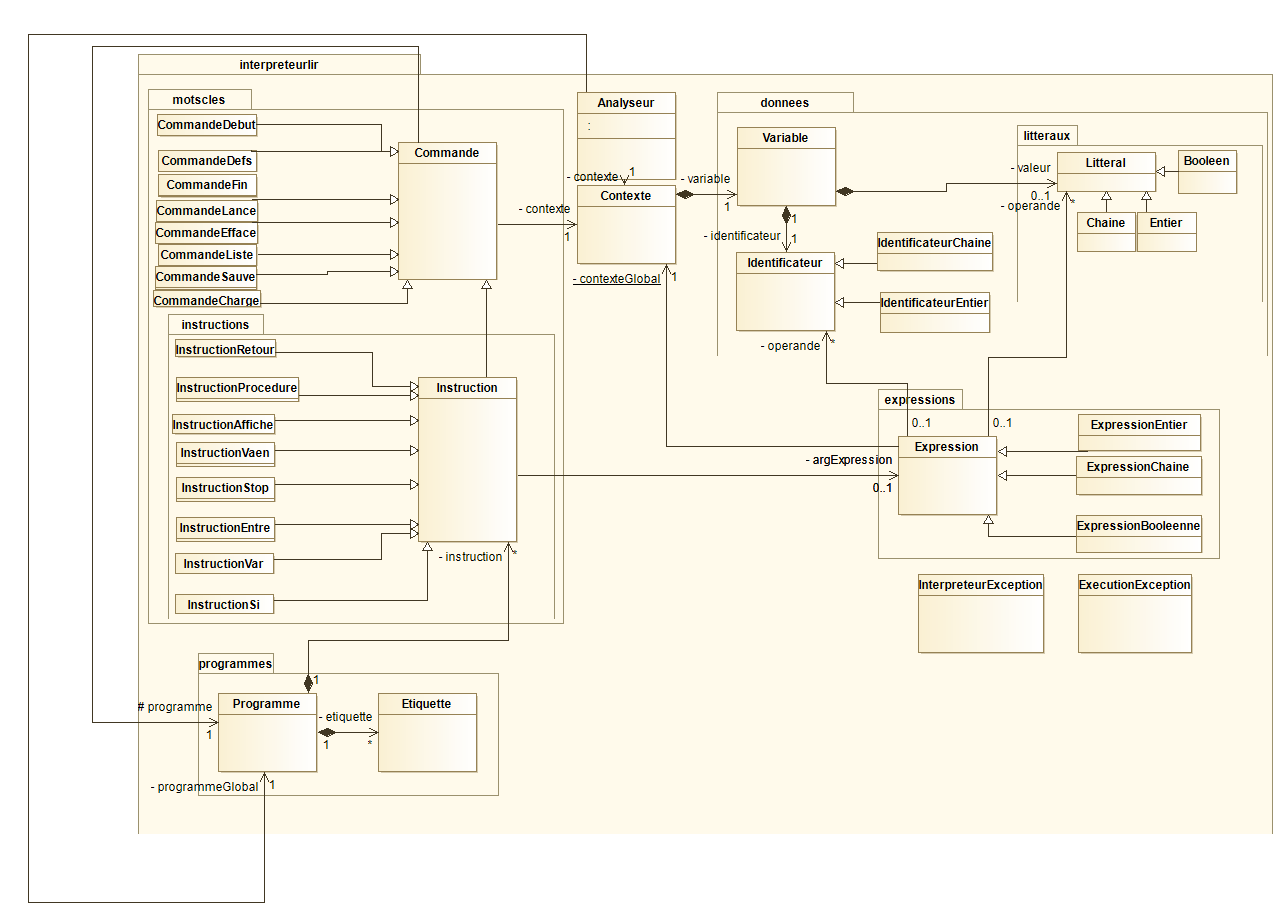
\includegraphics[scale=0.35]{fichiers/dossierPartieConception/img/COO/COO_prototype_3/Scéma général simplifié}\end{center}
\par Les commandes sauve et charge ont été ajoutés à la conception mais sont similaires aux autres commandes. Pareil pour l'instruction si vaen. Ce diagramme général permet de voir l'ensemble de la conception pour ce qui est des associations et généralisation des classes.

    \chapter{Projet final}

    \par Ce chapitre contient les diagrammes de classes représentant le logiciel codé. Les diagrammes de l'itération trois ont été complétés à partir du code pour ajouter les détails d'intégration dans le diagrammes (méthodes privées par exemple).

\section{Paquetage interpreteurlir.donnees(.litteraux)}
\begin{center}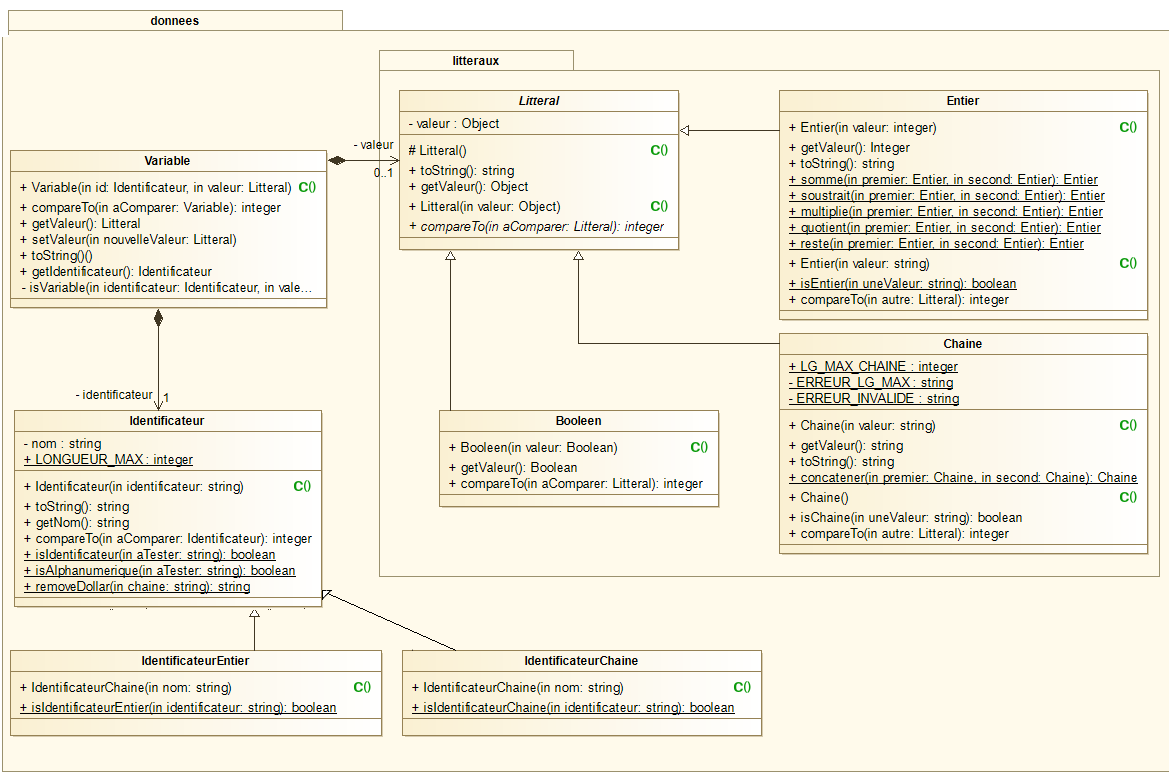
\includegraphics[scale=0.55]{./img/COO/PackageDonnees}\end{center}

\section{Paquetage interpreteurlir.expressions}
\begin{center}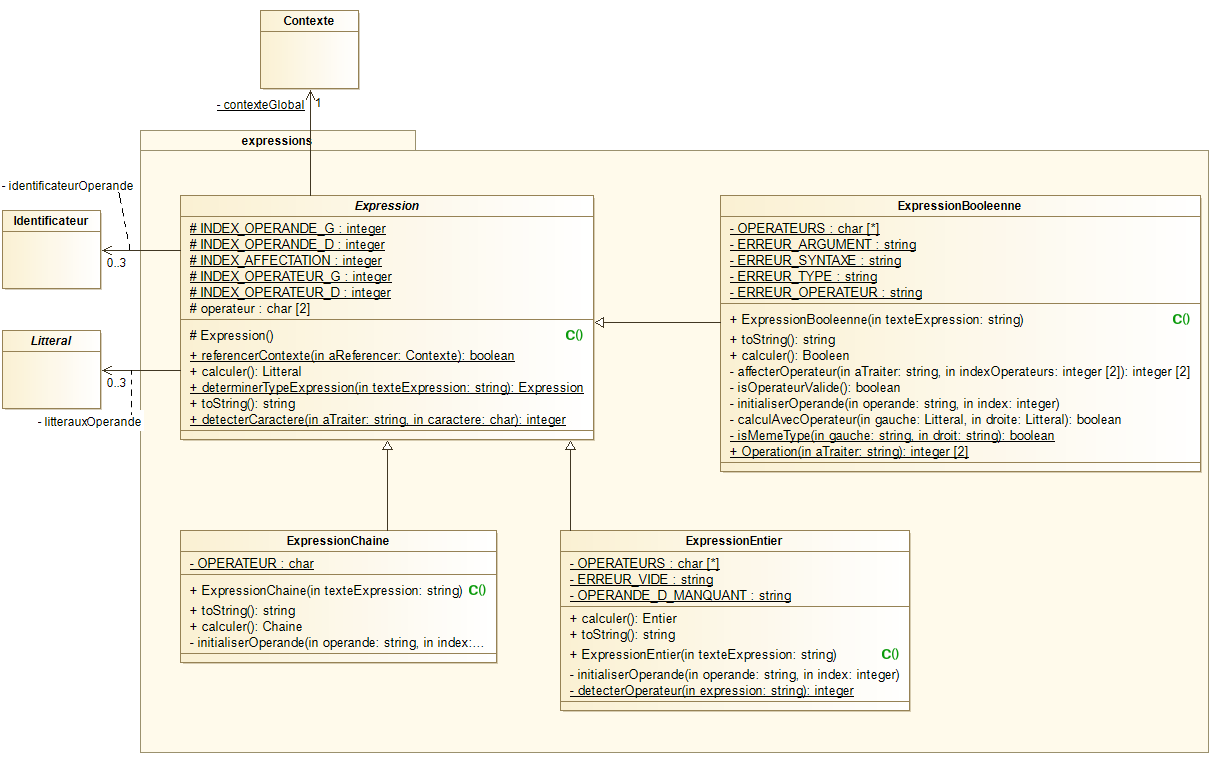
\includegraphics[scale=0.55]{./img/COO/PackageExpression}\end{center}

\section{Paquetage interpreteurlir.programmes}
\begin{center}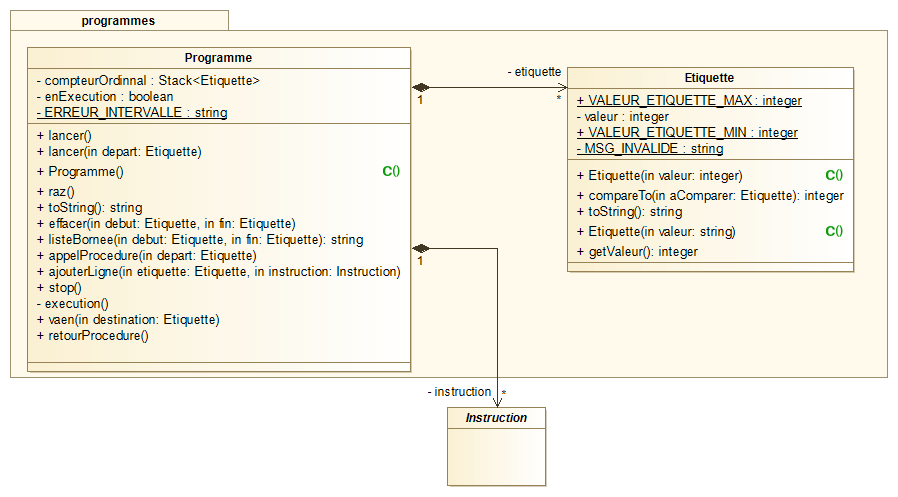
\includegraphics[scale=0.55]{./img/COO/PackageProgrammes}\end{center}

\section{Paquetage interpreteurlir.motscles}
\begin{center}\includegraphics[scale=0.60]{./img/COO/PackageMotscles}\end{center}

\section{Paquetage interpreteurlir.motscles.instructions}
\begin{center}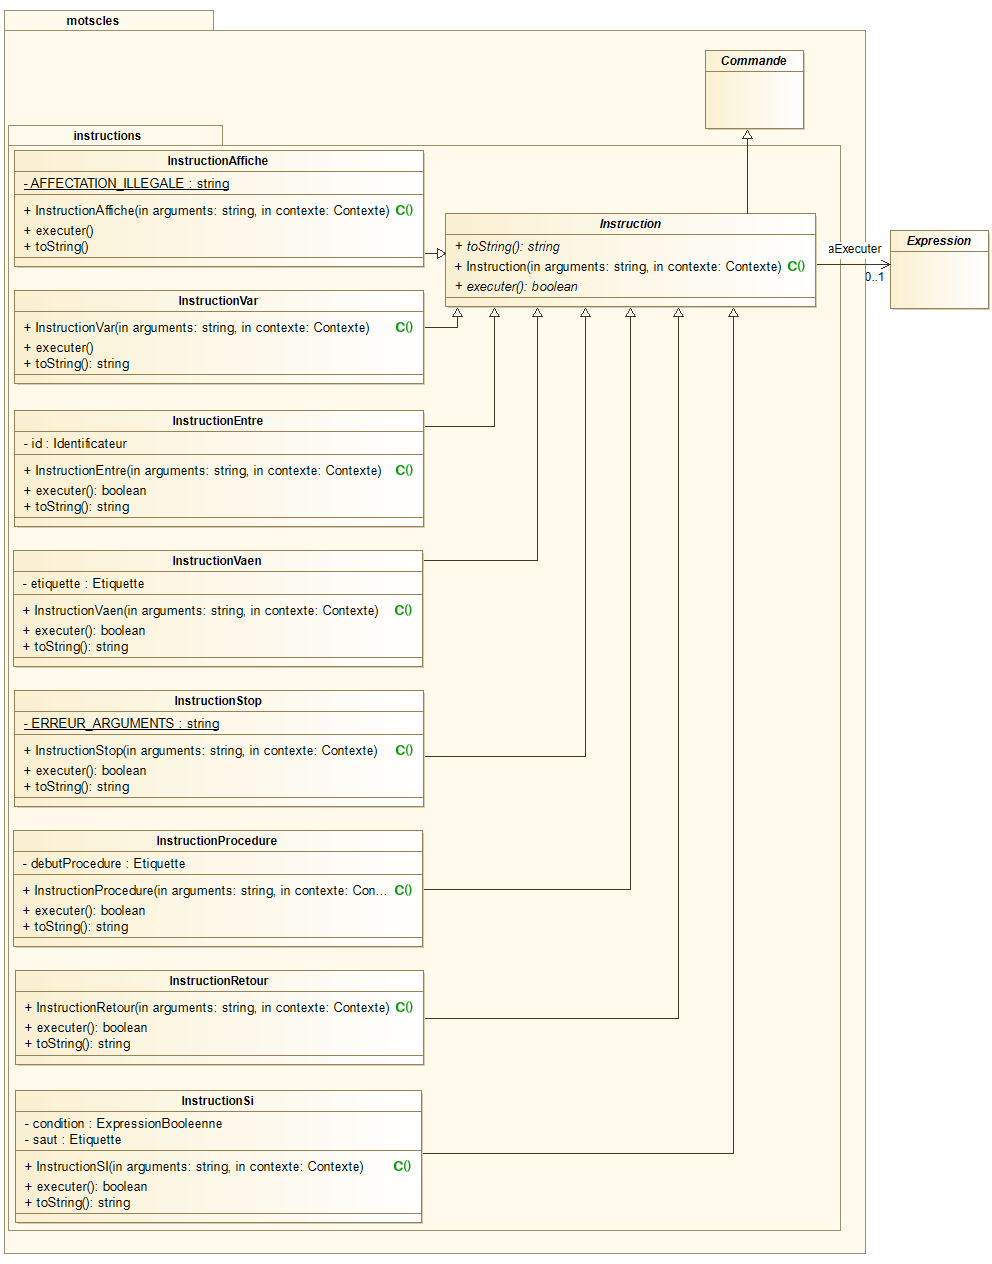
\includegraphics[scale=0.60]{./img/COO/PackageInstruction}\end{center}

\section{Paquetage interpreteurlir}
\begin{center}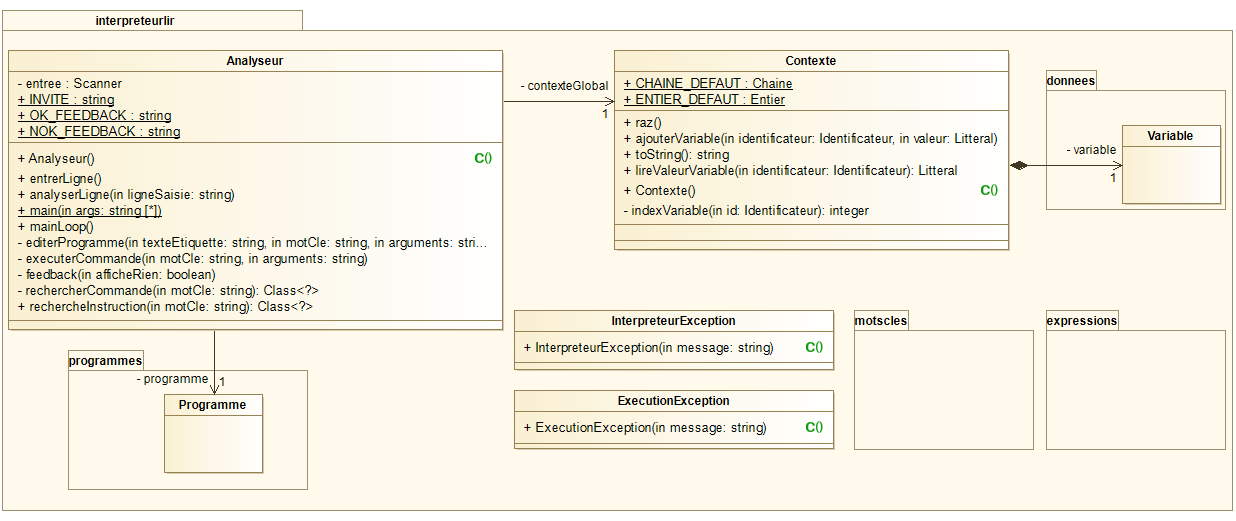
\includegraphics[scale=0.55]{./img/COO/PackageInterpreteurlir}\end{center}

\end{document}